\section{Discussion}
\label{sec:calibcant:discussion}

\subsection{Peak frequency}
\label{sec:calibcant:peak-frequency}

Since we went through the trouble of calculating the derivative of
$\PSD_f$ in \cref{eq:model-psd-df}, it's useful to also calculate the
frequency of the resonant peak.
\begin{align}
  0 &= \deriv{f}{\PSD_f}
    = \frac{2G_{1f}f_\text{max}}
           {\p({(f_0^2-f_\text{max}^2)^2 + \beta_f^2 f_\text{max}^2})^2}
      \p({2(f_0^2-f_\text{max}^2) - \beta_f^2}) \\
    &= 2(f_0^2-f_\text{max}^2) - \beta_f^2 \\
  f_\text{max}^2 &= f_0^2 - \frac{\beta_f^2}{2} \\
  f_\text{max} &= \sqrt{f_0^2 - \frac{\beta_f^2}{2}} \;,
  \label{eq:peak-frequency}
\end{align}
where we used $f\ne0$ during the large simplifying multiplication.  We
see that the peak frequency is shifted from $f_0$ depending on the
damping term $\beta_f$.  For overdamped cantilevers with large values
of $\beta$, the peak frequency will not have a real solution.%
%
\nomenclature[sr ]{$f_\text{max}$}{The frequency of the peak power in
  $\PSD_f$ (\cref{eq:peak-frequency}).}

\subsection{Propagation of errors}
\label{sec:calibcant:discussion:errors}

Extracting cantilever spring constants with \cref{eq:kappa} is great,
but the number you get is not much good if you can't estimate its
accuracy.  We can find the effect of measurement and fitting errors on
the calculated $\kappa$ using Taylor expansions\citep{ku66}.  To the
first order,

\begin{equation}
  f(\vect{x}) \approx f_0 + \sum_i^n \p({\deriv{x_i}{f}(x_i - x_{i0})}) \;.
\end{equation}

To applying this to \cref{eq:kappa}, we need the derivatives
\begin{align}
  \deriv{\sigma_p}{\kappa}
     &= \deriv{\sigma_p}{}\p({\frac{\sigma_p^2 k_BT}{\avg{V_p(t)^2}}})
     = \frac{2\kappa}{\sigma_p} \\
  \deriv{T}{\kappa} &= \frac{\kappa}{T} \\
  \deriv{\avg{V_p(t)^2}}{\kappa} &= \frac{-\kappa}{\avg{V_p(t)^2}} \;,
\end{align}
where I have used $\avg{V_p(t)^2}$ directly to support alternative
variance extraction models (\cref{sec:calibcant:vibration}).

Our measurements of $\sigma_p$, $T$, and $\avg{V_p(t)^2}$ are
independent and therefore uncorrelated.  This lets us estimate
standard deviation of $\kappa$ from the standard deviation of the
measured parameters\citep{ku66}.

\begin{align}
  \sigma_\kappa &\approx \sqrt{
      \p({\deriv{\sigma_p}{\kappa}})^2 \sigma_{\sigma_p}^2 +
      \p({\deriv{T}{\kappa}})^2 \sigma_{T}^2 +
      \p({\deriv{\avg{V_p(t)^2}}{\kappa}})^2 \sigma_{\avg{V_p(t)^2}}^2
      } \\
    &\approx \sqrt{
      \frac{4\kappa^2}{\sigma_p^2} \sigma_{\sigma_p}^2 +
      \frac{\kappa^2}{T^2} \sigma_{T}^2 +
      \frac{\kappa^2}{\avg{V_p(t)^2}} \sigma_{\avg{V_p(t)^2}}^2
      } \\
  \frac{\sigma_\kappa}{\kappa} &\approx \sqrt{
      4\p({\frac{\sigma_{\sigma_p}}{\sigma_p}})^2 +
      \p({\frac{\sigma_{T}}{T}})^2 +
      \p({\frac{\sigma_{\avg{V_p(t)^2}}^2}{\avg{V_p(t)^2}}^2})
    }
\end{align}

By repeating each experiment (surface bumps, temperature readings, and
thermal vibrations) several times, we can estimate the statistical
uncertainty in each parameter (\cref{fig:calibcant:statistics}).
Values for $\sigma_p$ and $\avg{V_p^2}$ are quite sensitive to the
location of the laser spot on the cantilever, so they can vary over
large time scales as the microscope alignment drifts (e.g.~due to
thermal expansion as the room warms up).  However, the calculated
value for $\kappa$ should not vary significantly.

For example, on a recent calibration run\footnote{2013-02-07T08-20-46}
I measured $\sigma_p=35.68\pm0.87\U{V/$\mu$m}$,
$T=298.151\pm0.033\U{K}$, and $\avg{V_p^2}=96.90\pm0.99\U{mV$^2$}$,
which gives $\kappa=54.1\pm2.7\U{mN/m}$.  These numbers are very
similar to those obtained with a different cantilever from the same
batch measured a month later (\cref{tab:calibcant:stability}).  The
uncertainty contributions from each term are
\begin{align}
  4\p({\frac{\sigma_{\sigma_p}}{\sigma_p}})^2 &= 2.38\E{-3}\U{N$^2$/m$^2$} \\
  \p({\frac{\sigma_{T}}{T}})^2 &= 1.29\E{-8}\U{N$^2$/m$^2$} \\
  \p({\frac{\sigma_{\avg{V_p(t)^2}}^2}{\avg{V_p(t)^2}}^2})
    &= 1.04\E{-4}\U{N$^2$/m$^2$}
\end{align}
The size of the thermal vibration is
$\sqrt{\avg{V_p^2}}/\sigma_p\approx2.8\U{\AA}$ with forces on the
order of $\kappa\sqrt{\avg{V_p^2}}/\sigma_p\approx15\U{pN}$.

In this particular run, most of the uncertainty in $\kappa$ comes from
$\sigma_{\sigma_p}$, with some from $\sigma_{\avg{V_p(t)^2}}$.  To add
uncertainty comparable to the photodiode sensitivity contribution, the
temperature variance would have to be
\begin{equation}
  \sigma_T = \frac{\sigma_{\sigma_p}}{\sigma_p}\cdot T
    \approx \frac{2\cdot 0.87}{35.68} \cdot 298.151\U{T}
    \approx 15\U{K} \;.
\end{equation}
This is a large enough window that simply using room temperature (or
even a hard-coded $300\U{K}$) should not introduce excessive error in
the calculated $\kappa$.

\begin{figure}
  \begin{center}
    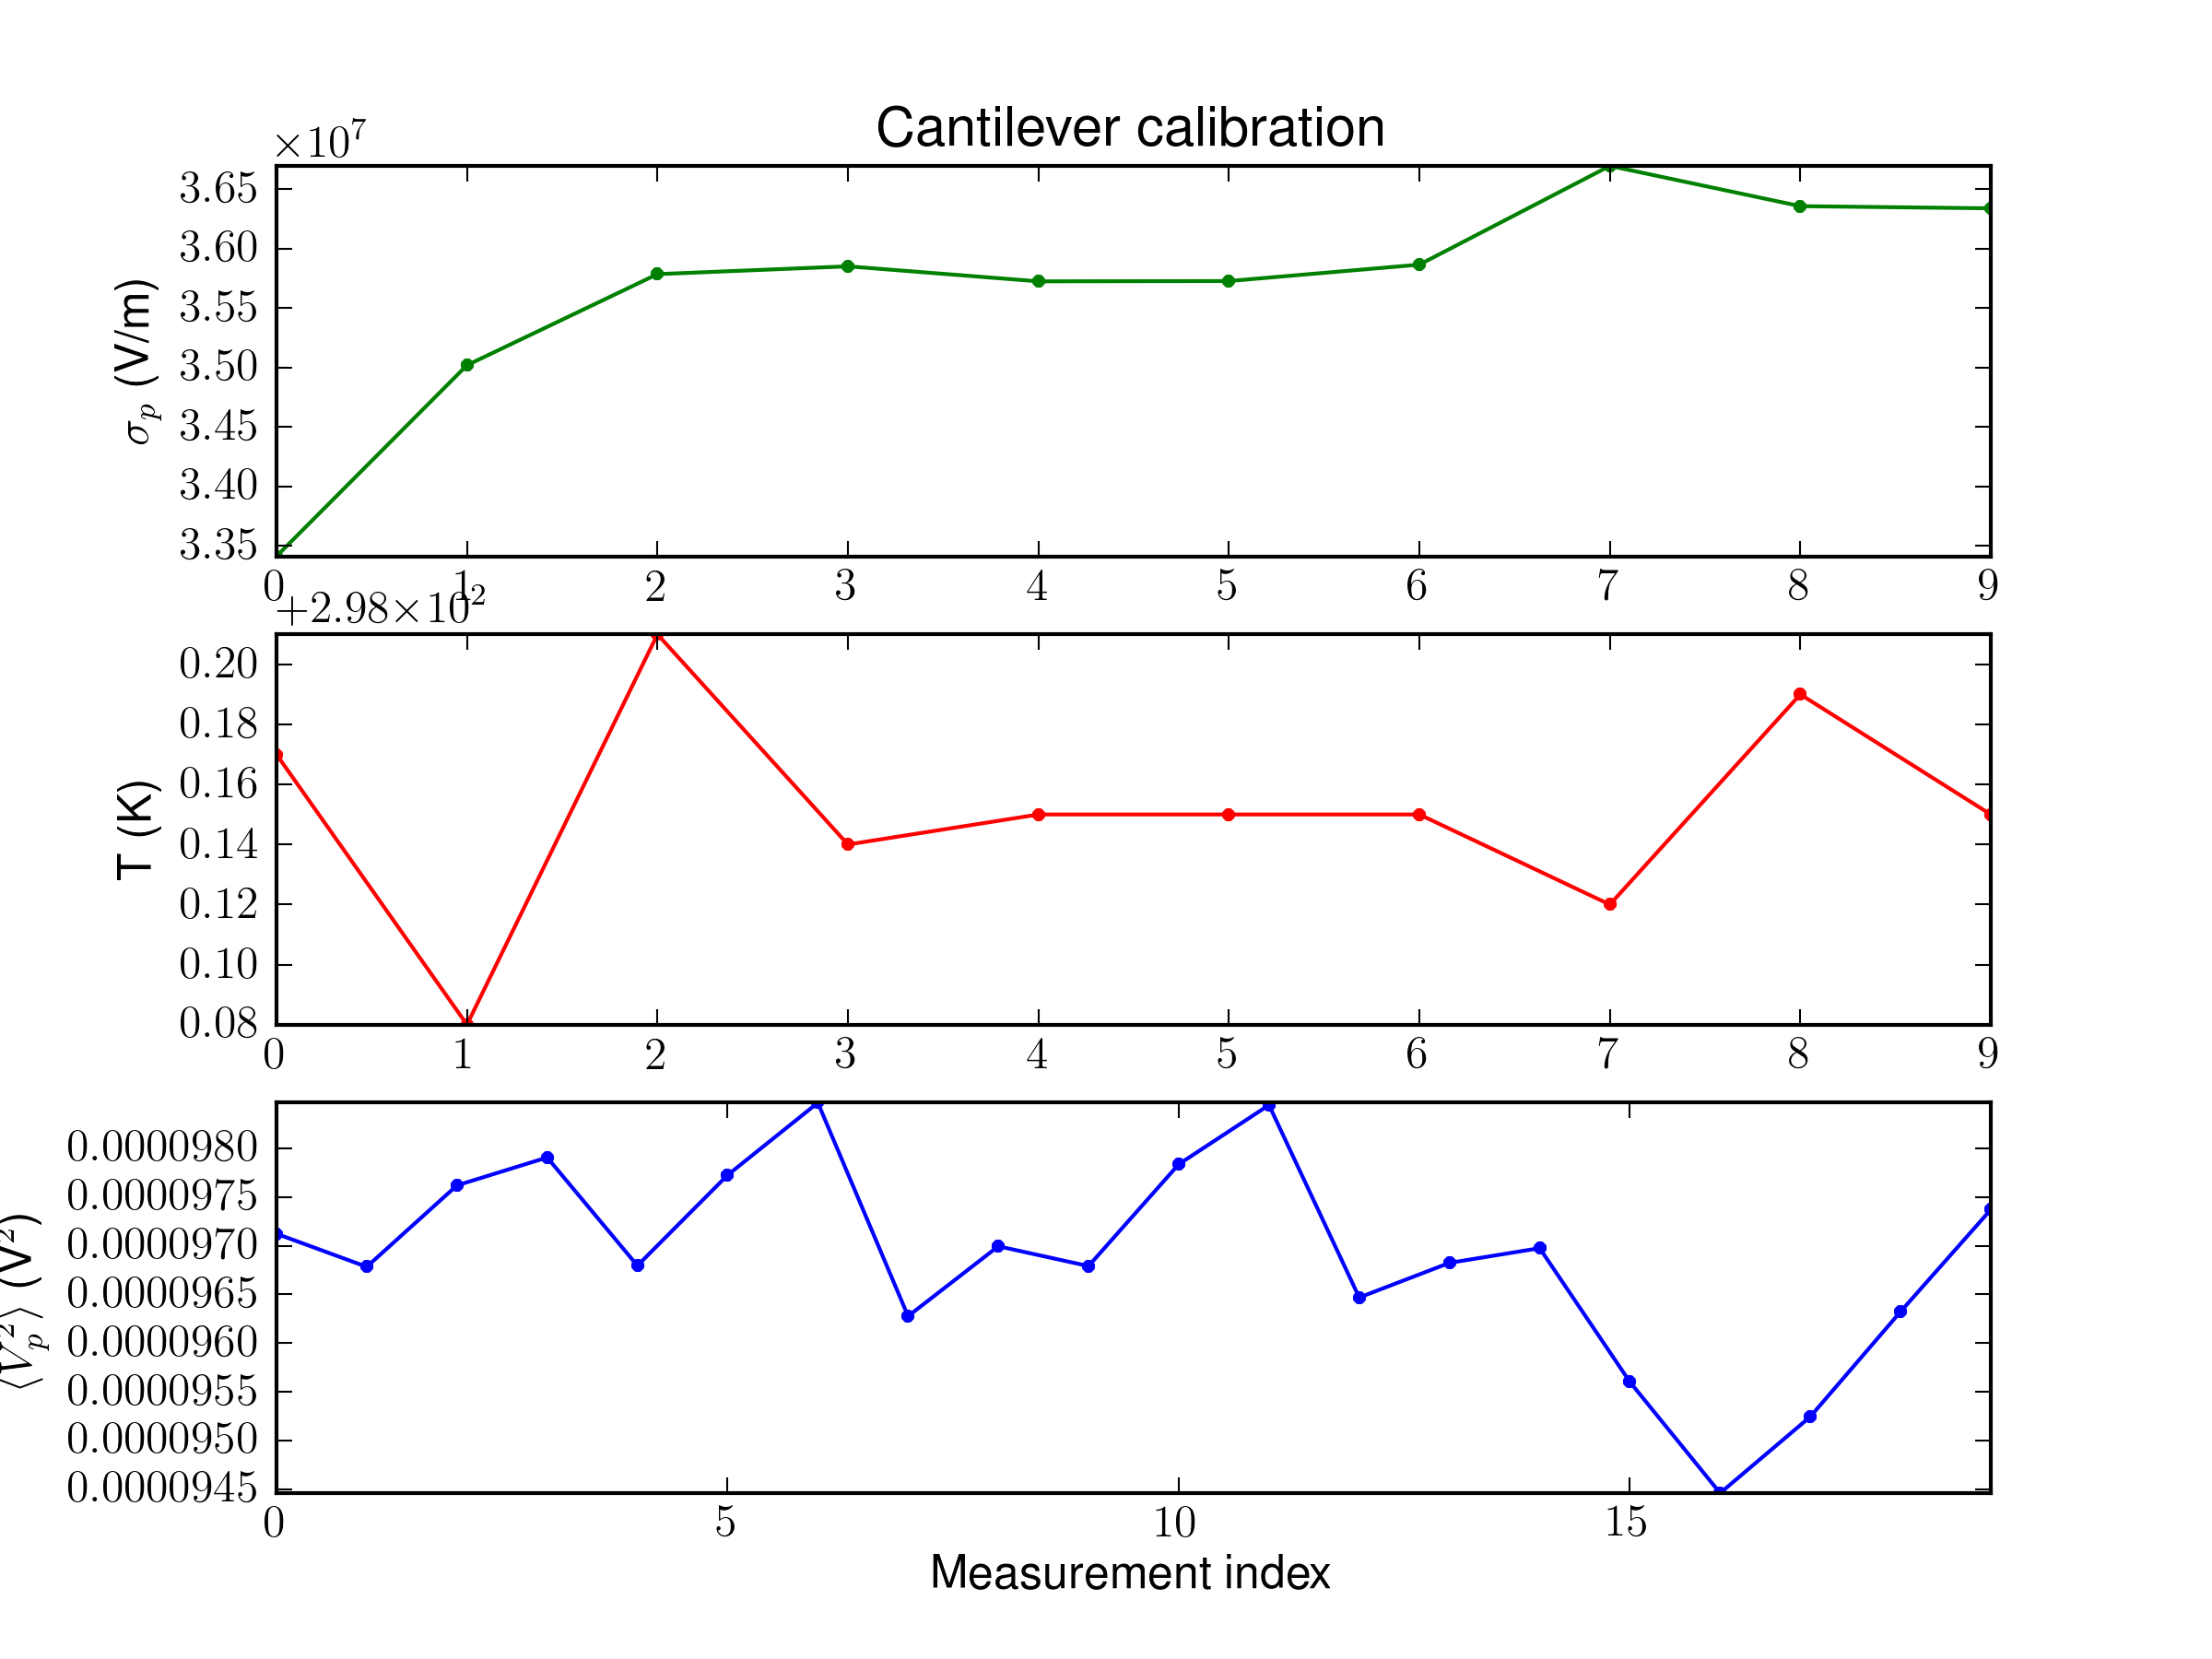
\includegraphics[width=0.8\textwidth]{figures/calibcant/statistics}
    \caption{Estimating the statistical uncertainty of the calculated
      cantilever spring constant $\kappa$ through repeated
      measurements.\label{fig:calibcant:statistics}}
  \end{center}
\end{figure}

\begin{table}
  \begin{center}
    \begin{tabular}{c c S[table-format=3.3] S[table-format=1.3]
                        S[table-format=3.3] S[table-format=1.3]}
      \toprule
      \multicolumn{2}{c}{Timestamp:} &
      \multicolumn{2}{c}{2013-03-03T16-37-12} &
      \multicolumn{2}{c}{2013-03-04T12-21-54} \\
      \midrule
      Quantity & Units & {Mean} & {Std.~Dev.} & {Mean} & {Std.~Dev.} \\
      \midrule
      $\sigma_p$    & \bareU{V/$\mu$m} & 46.22   & 0.76  & 41.30   & 0.21 \\
      $T$           & \bareU{K}        & 296.302 & 0.021 & 294.272 & 0.022 \\
      $\avg{V_p^2}$ & \bareU{mV$^2$}   & 108.3   & 1.1   & 105.5   & 2.16 \\
      $\kappa$      & \bareU{mN/m}     & 67.3    & 2.5   & 65.6    & 1.5 \\
      \bottomrule
    \end{tabular}
    \caption{Measured spring constant calibration parameters (mean and
      standard deviation) for a single cantilever on two consecutive
      days.  The measured parameters have changes slightly because the
      laser alignment and buffer temperature drift over time, but the
      measured $\kappa$ are not significantly different ($p=0.9$, as
      measured with a two-tailed Welch's
      $t$-test\citep{welch38,welch47}).\label{tab:calibcant:stability}}
    % Using Welch's t test
    %     http://en.wikipedia.org/wiki/Welch%27s_t_test
    %   from math import sqrt  # using Python in the following
    %   x1 = 67.3
    %   v1 = 2.5**2
    %   n1 = 10    # sortof :p
    %   x2 = 65.6
    %   v2 = 1.5**2
    %   n2 = 10
    %   t = (x1 - x2) / sqrt(v1/n1 + v2/n2)
    %     = 1.8
    % Degrees of freedom with the Welch-Satterthwaithe equation
    %   df = (v1/n1 + v2/n2)**2 / ( (v1/n1)**2/(n1-1) + (v2/n2)**2/(n2-1) )
    % Test null hypothesis that means are equal (two-tailed t)
    %     http://en.wikipedia.org/wiki/Two-tailed_test
    %   from scipy.stats.mstats import betai
    %   p = betai(0.5*df, 0.5, float(df) / (df + t*t))
    %     = 0.09
    % With arrays, we could have used scipy.stats.mstats.ttest_ind().
  \end{center}
\end{table}

\subsection{Archiving experimental data}
\label{sec:calibcant:discussion:data}

Scientific data is not thrown away after analysis.  Organizations may
have standards for archival, and many journals require supporting data
to be available on request after publication or archived in public
databases\citep{pnas-data-archival,nature-data-archival}.  Both the
raw data and the experimental parameters used to collect need to be
preserved, but managing this manually is tedious and error prone.  Lab
notebooks rarely contain \emph{all} of the parameters used to collect
and analyze a particular calibration.  Data collected with
\calibcant\ is saved in \citetalias{hdf5} with the full configuration
(\cref{sec:pyafm:h5config}), bundling all of the information together
in a single file.

One minor drawback to this approach is that configuration information
(which is not likely to change often) is duplicated between
calibration runs.  While this uses some extra disk space, the overhead
is small.  The full calibration datafile weighs in at $3.4\U{MB}$,
while the calibration section alone is just $37\U{kB}$ (1\% of the
total).

Besides the benefit of having a self contained file, HDF5 provides
efficient support for large arrays of typed data (such as the unsigned
16-bit values from our DACs and ADCs), which is not possible with many
other open file formats.  The HDF libraries are supported by the
non-profit HDF Group with a 20 year development
history\citep{hdf-group} and many users\citep{hdf-users}.  This
suggests that HDF will be around for the long haul, and if it is
eventually phased out, that there will be a number of well funded
organizations interested in developing migration plans.
